\section{Dynamic Provisioning of Web Services for Simulation Workflows}
\label{related:dynamic}

\textcolor{red}{VERWIRRUNG}

\citeauthor{provisioning:dynamic} found some problems with the architecture proposed in \autoref{related:ondemand}.
The original architecture assumes that only one provisioning engine is used.

that every provisioning engine knows how to communicate with the service repository to get the information and resources it need to provision a service.
While this might be true for some provisioning engines, it's certainly not true for all of them.
This problem is further amplified because there are no standards defined for such a service repository.

Another assumption of the original architecture is that a provisioning engine always understands the format of the service packages provided by the service repository.
Different provisioning engines use different formats which are in general not compatible.
If provisioning engines would all use a standardized format (like CSAR), this would not be a problem, but that isn't the case.

\begin{figure}[!htbp]
	\centering
	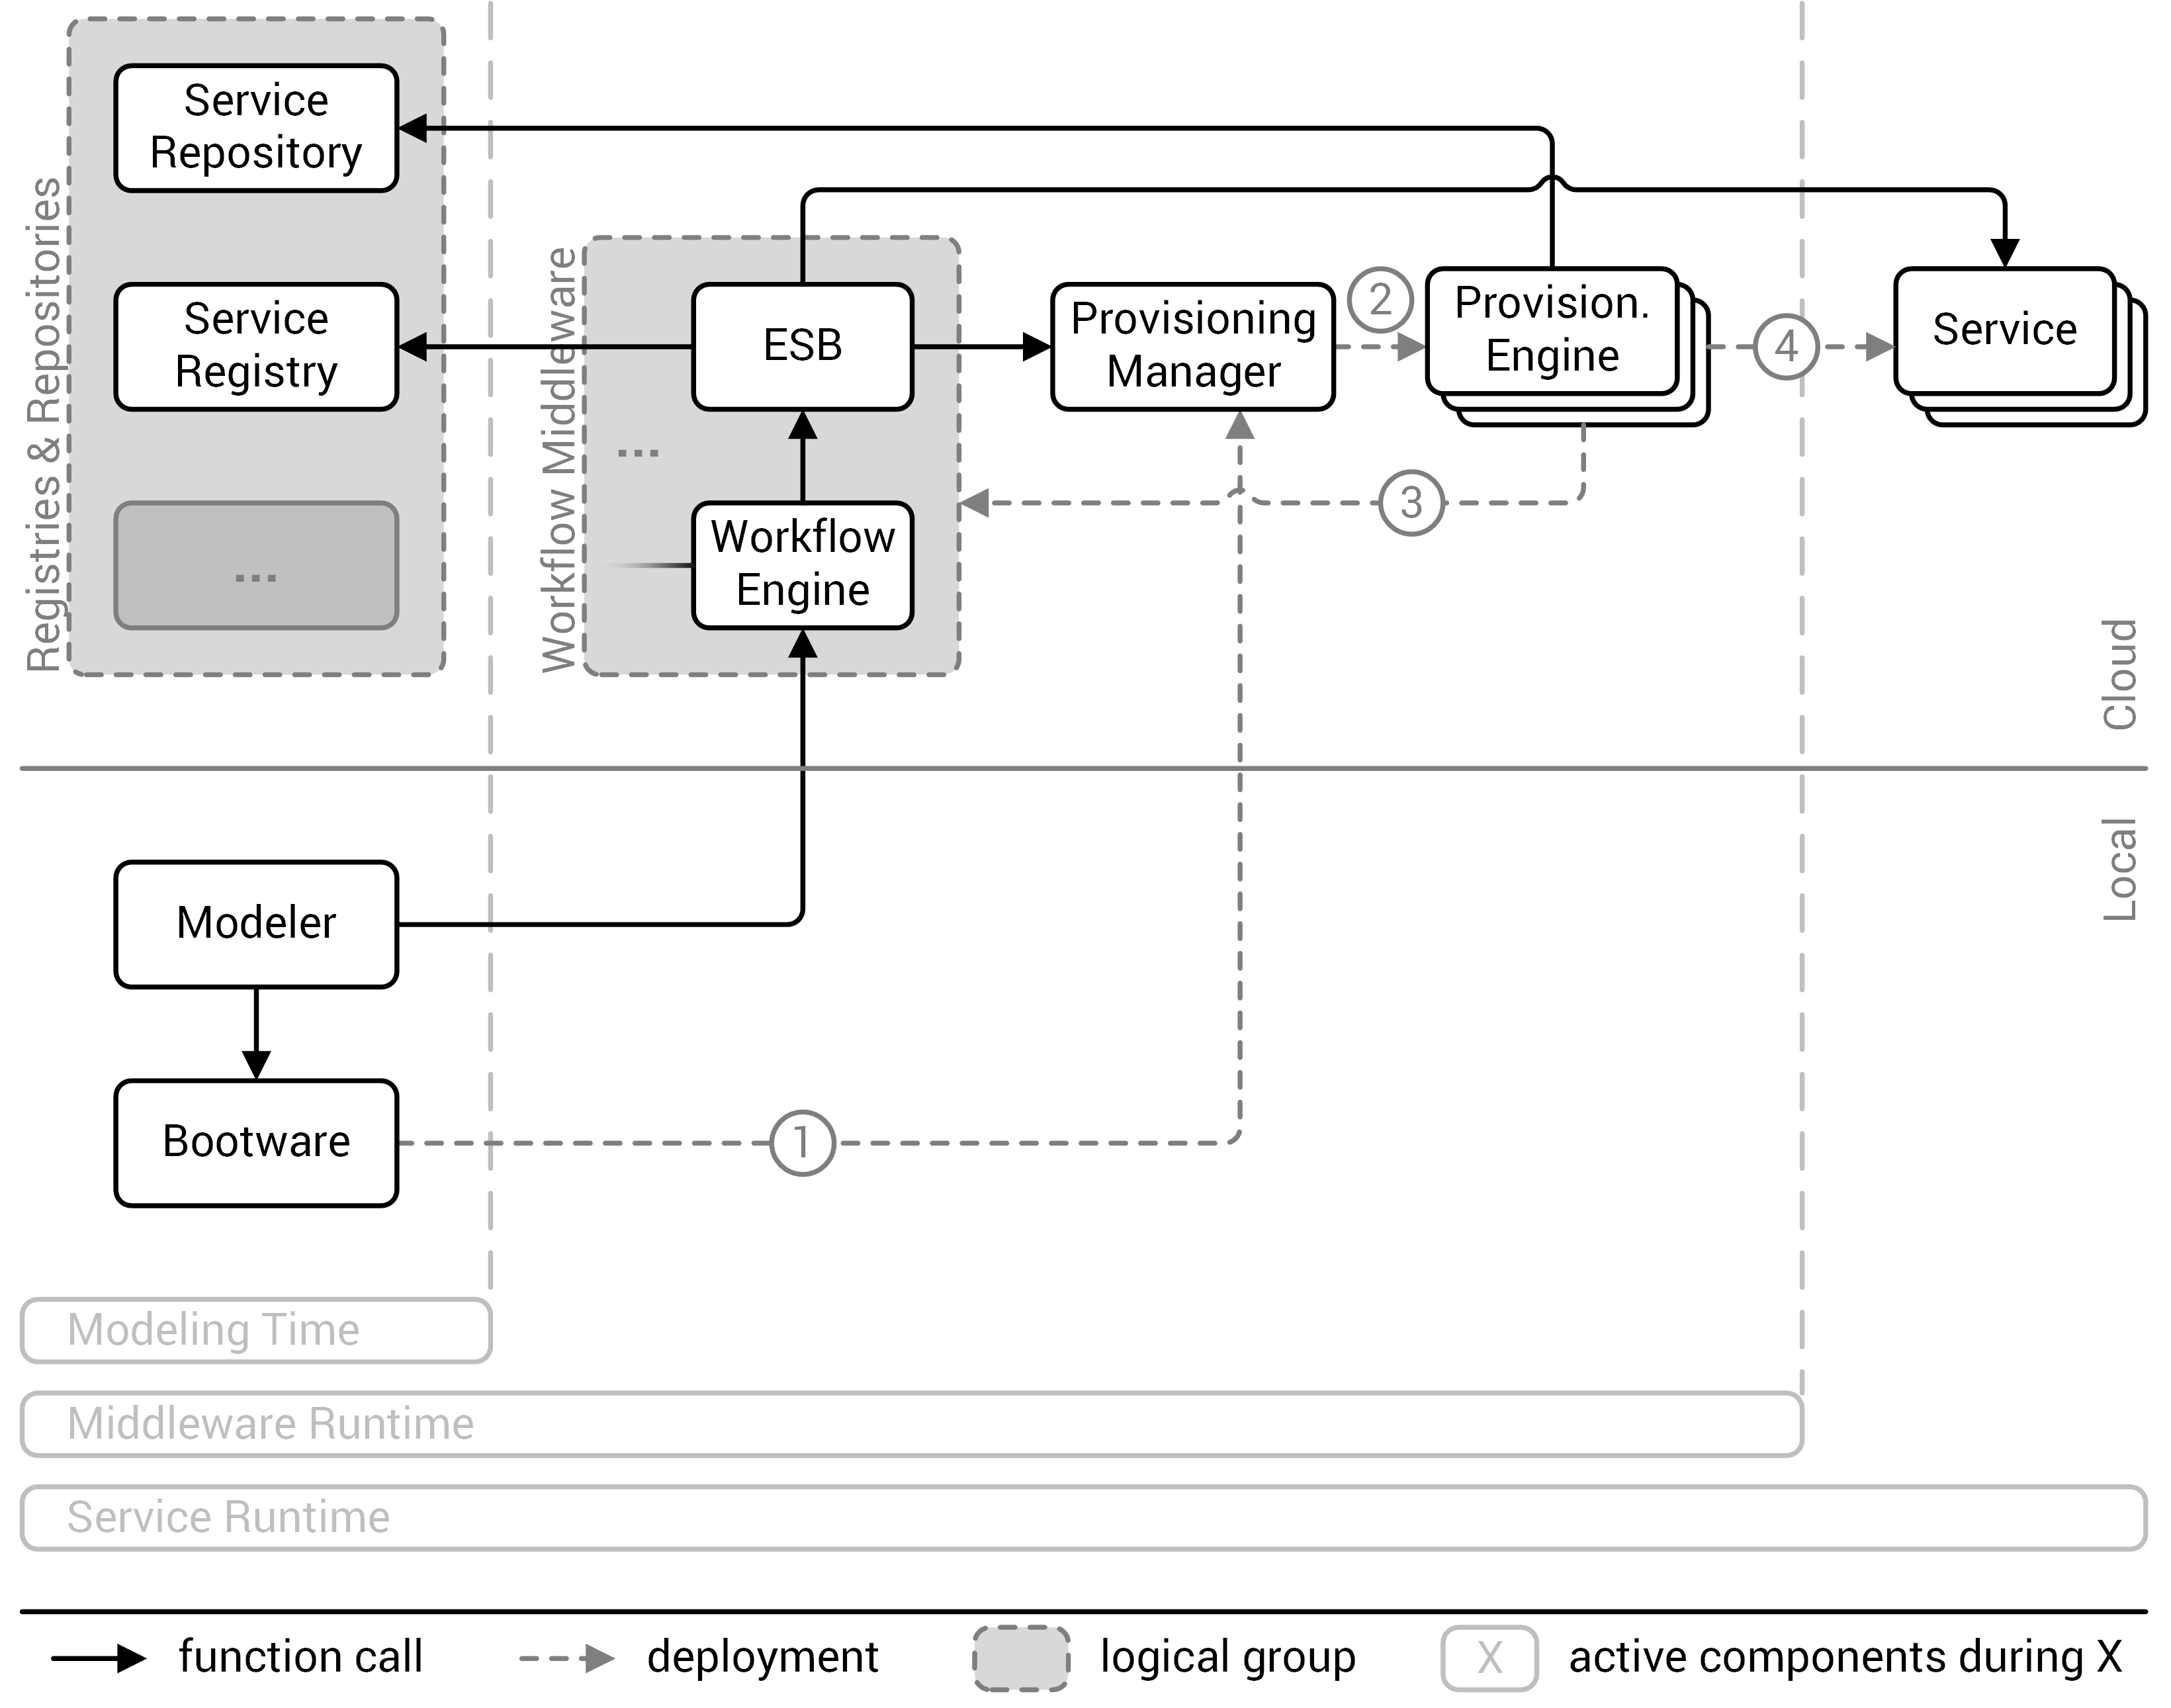
\includegraphics[resolution=600]{related/assets/valeri_architecture}
	\caption{Extended architecture with added provisioning manager~\autocite[based on][]{provisioning:dynamic}}
	\label{image:valeri_architecture}
\end{figure}

\citeauthor{provisioning:dynamic} further refines the previously shown middleware architecture by adding a provisioning manager as intermediary between the \nom{Enterprise Service Bus}{ESB} and the provisioning engines~\autocite{provisioning:dynamic}.
This addition improves the original architecture in three aspects.

The \textcolor{red}{ESB} can now use the stable interface of the provisioning manager to trigger provisioning engines instead of calling those provisioning engines directly.
The provisioning manager handles the differences between the provisioning engines.
This makes it also possible to use multiple different provisioning engines during one workflow execution.

The provisioning manager also handles the communication with the service registry or possibly multiple service registries for different provisioning engines.

The provisioning manager could also translate different service distribution formats so that provisioning engines could be used with formats that they don't support


